
La dernière alerte modélisée est le cas dit du \enquote{fil rouge} que
nous avions présenté dans le premier chapitre de cette thèse. Comme
nous l'avions indiqué lors de sa première présentation, le \emph{fil
  rouge} est une alerte particulière, contenant de nombreux indices
très imprécis et incertains. Par conséquent la \ac{zir} est
extrêmement étendue.


\subsection{Présentation de l'alerte}
\label{subsec:9-4-1}

Le fil rouge est une alerte composée de XX \emph{indices de
  localisation.}


Faute d'enregistrement audio, le fil rouge n'a pas été retranscrit,
les indices dont nous disposons (et qui avaient été présentés dans le
\autoref{chap:01}) ont donc été directement saisis par le secouriste.
%
de ce fait, le \emph{fil rouge} est une alerte assez différente des
précédentes, puisque XXX n'est pas
%
Le traitement du \emph{fil rouge} est donc plus proche du traitement
opérationnel qui sera réellement effectué lors du traitement d'une
alerte.


Pour le cas du \emph{fil rouge} nous ne disposons pas de
l'enregistrement audio et donc de son verbatim, les indices ayant déjà 
été synthétisés par les secouristes. Les les avions déjà présentés
dans le \autoref{chap:01}.
%
Pour rappel voici la synthèse de l'alerte qui nous a été donnée par
les secouristes :
%
\begin{enumerate}
\item La victime est partie de Bourg d'Oisans, à pied, sur chemin, en
  direction d'une station de ski.
\item La victime a marché plusieurs heures.
\item La victime a chuté de plusieurs mètres.
\item La victime voit une partie de plan d'eau.
\item La victime est sous une route et entend des véhicules.
\item La victime est sous une ligne électrique 3 brins.
\item La victime vient de passer du soleil à l'ombre.
\end{enumerate}


Comme on peut le remarquer, ces indications 

La première de ces sept descriptions donne beaucoup d'informations sur
le trajet suivit par la victime jusqu'à sa position actuelle. On
connait sont point de départ, clairement identifié, la destination
visée, une station de ski inconnue et son mode de déplacement, à pied
sur un chemin. 

Le second élément de cette alerte, \enquote{La victime a marché
  plusieurs heures}, nous donne une indication de la durée du
déplacement de la victime. 


Le troisième élément de l'alerte nous indique que la victime a chuté
de plusieurs mètres. Prise sous cette forme, cette description n'est
pas transformable en un indice de localisaiton et aucune relation de
localisation ne permet de l'exprimer. Il est cependant possible
d'interpréter cette information, de manière à en construire un indice
de localisation. En effet, les trois premières informations nous
renseignent sur le trajet qu'a suivi la victime, jusqu'à arriver a sa
position actuelle, on connait son point de départ, sa destination
potentielle, son mode de déplacement, \emph{etc.} Grace à ces
précédentes informations on peut supposer, avec une relative
certitude, que la lors de sa chute la victime se déplaçait sur un
chemin. Ainsi s'il nous est impossible de construire directement une
\ac{zlc} grâce à l'information \enquote{J'ai chuté de plusieurs
  mètres}, il nous est en revanche possible de dériver de cette
information un indice de localisation exprimant la position actuelle
de la victime, par rapport au chemin dont elle vient de chuter.



Vient ensuite la quatrième description où la victime indique qu'elle
voit une partie de plan d'eau.
%
Il est ici assez facile d’identifier la relation de localisation
adaptée à la modélisation de cette relation de localisation



Dans la cinquième descrition, la victime indique qu'elle est sous une
route


Dans la sixième description, la victime indique qu'elle se situe sous
une ligne électrique trois brins.
%
Nous avons déjà présenté ce cas, notamment dans le \autoref{chap:06}
où nous comparions les différentes implémentations de la théorie des
sous-ensembles flous pour représenter des zones de localisation. Si
nous n'avions pas encore présenté les différentes relations de
localisation, définies dans l'ontologie des relations de localisation,
nous avions déjà expliqué que cette description nécessitait que la
relation de verticalité entre le \emph{site} et la \emph{cible} soit
contrainte selon l'axe horizontal. Dit autrement, il est ici
nécessaire d'être proche du \emph{site} et à une altitude inférieure
du \emph{site} pour que l'on puisse affirmer qu'une position soit
\enquote{sous} le \emph{site.} Une relation de localisation,
\onto{Sous\-Proche\-De} a spécifiquement été définie pour modéliser ce
type de relation.


Au terme de l'analyse de l'alerte on dispose donc de 6 indices de
localisation à spatialiser:
% 
\begin{enumerate}
\item \label{ind:fr1} La victime est en direction de
  % 
\item \label{ind:fr2} La victime est
  \onto[orl]{A\-Temps\-De\-Marche\-De} \emph{Bourg-d'Oisans} 
  % 
\item \label{ind:fr3} La victime est \onto[orl]{Sous\-Proche\-De} un
  chemin
  % 
\item \label{ind:fr4} La victime voit
  % 
\item \label{ind:fr5} La victime est \onto[orl]{Sous\-Proche\-De} une
  route
  % 
\item \label{ind:fr6} La victime est \onto[orl]{Sous\-Proche\-De} une
  ligne électrique trois brins
\end{enumerate}



\subsection{Modélisation de l'alerte}
\label{subsec:9-4-2}

La \ac{zir} définie pour cette alerte est une zone de
\SI{625}{\kilo\meter\squared}

\begin{figure}
  \centering
  \begin{tikzpicture}
  \tikzset{et/.style={above,font=\footnotesize\vphantom{Ag}}}
  % 
  \node[inner sep=0pt, anchor=south west] (image) at (0,0){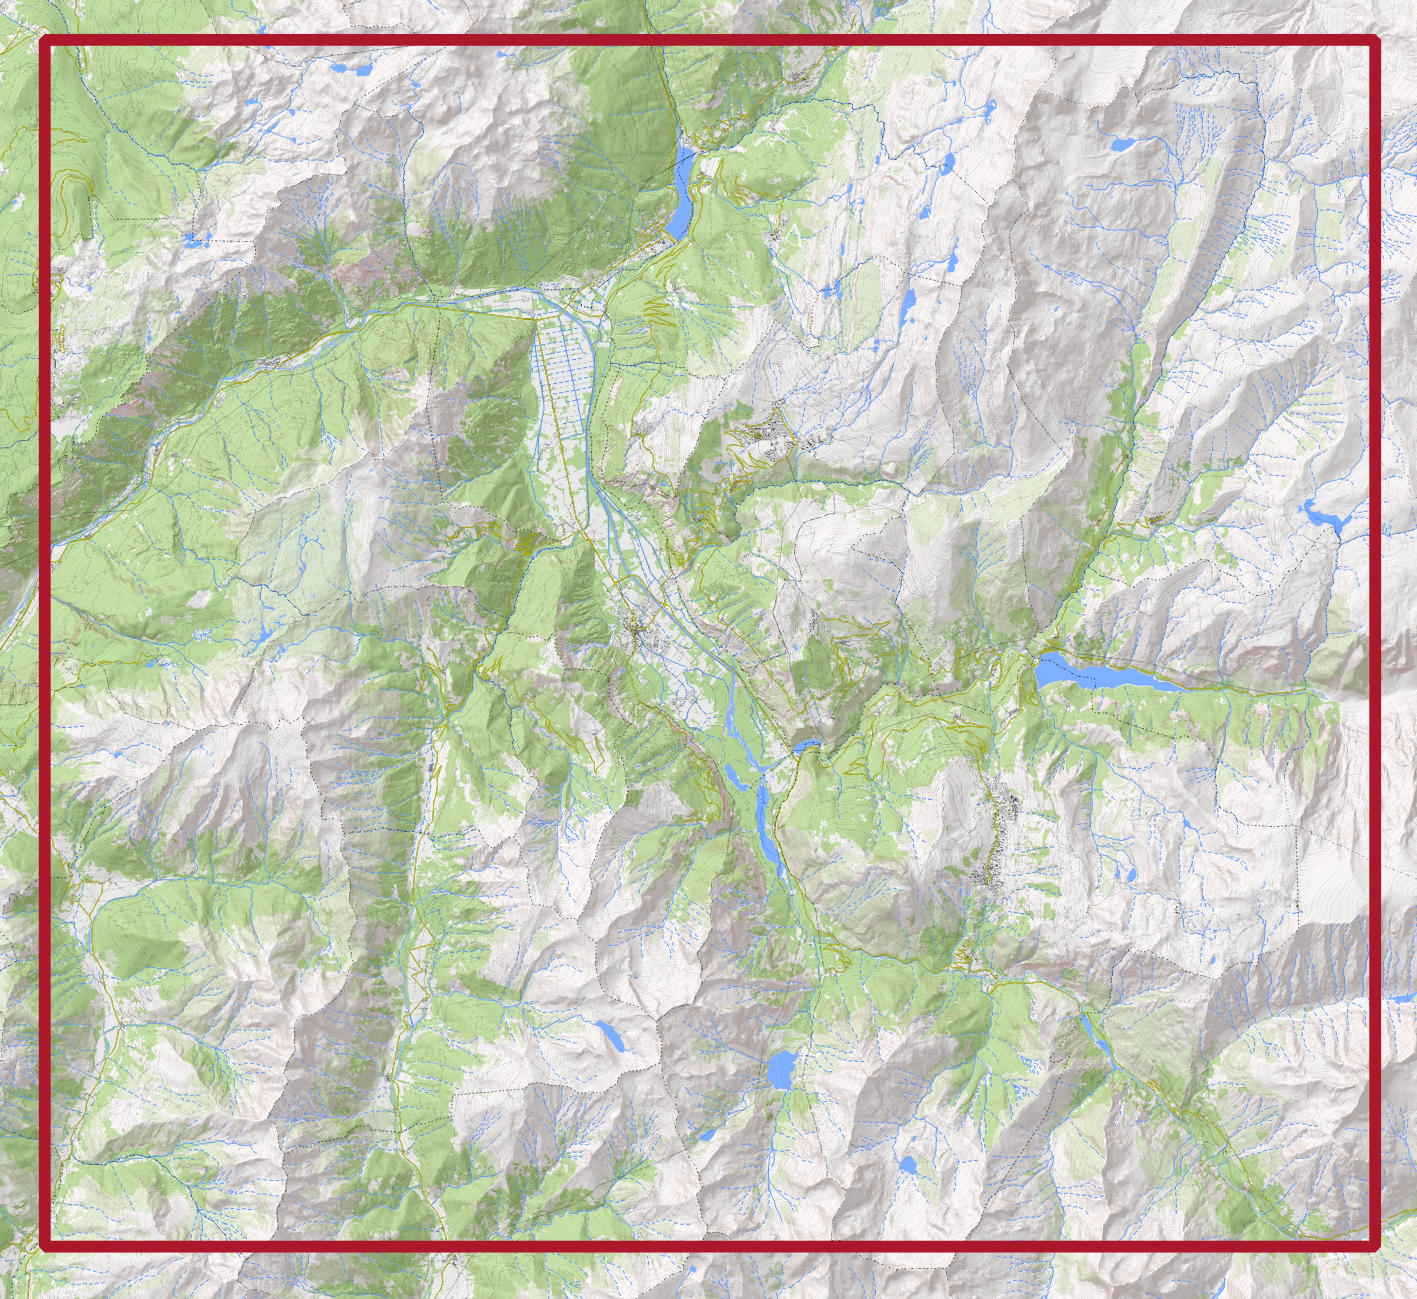
\includegraphics{./figures/ZIR_fil_rouge.png}};
  % 
  \begin{scope}
    \node (P2) at ([yshift=-.5cm]image.south east) {};
    \node (P1) at ([yshift=-.5cm]image.south west) {};
    % 
    \node (rect) [anchor=north west, minimum width=1cm,minimum
    height=.25cm] at ([yshift=-.25cm]P1) {}; \path[draw=RdBu-9-1, line
    width=1mm](rect.west) --([xshift=-1ex]rect.south) -- ([xshift=1ex]rect.north)
    -- (rect.east);
    % 
    \node[anchor=west, font=\tiny\vphantom{Ag}, text width = 4cm] at
    ([xshift=1ex]rect.east) {Limite de la \ac{zir}};
    % Échelle
    % Échelle
    \draw[-] (P2 |- -1cm,-1cm) --++ (-1,0) node[et,pos=.5] {\SI{2}{\kilo\meter}};
    % Légende détaillée
    \path (P1) -- (P2) node[pos=.5, yshift=-1cm] {\tiny Pour la légende détaillée du fond topographique voir \autoref{anx:topo_leg}. Sources: BD TOPO 2018, BD ALTI 2018.}; 
  \end{scope}
\end{tikzpicture}
  \caption{Zone initiale de recherche pour le \emph{fil rouge}}
  \label{fig:zir_fil_rouge}
\end{figure}

\subsubsection{La victime est \protect\onto[orl]{Sous\-Proche\-De} un chemin}

L'indice de localisation suivant (\ref{ind:fr3}) utilise la relation
de localisation \onto[orl]{Sous\-Proche\-De} que nous avions déjà
présenté, sans la nommer, dans le \autoref{chap:06}. Cette relation de
localisation n'est pas atomique, elle est définie comme la conjonction
de deux relations de localisation atomiques,
\onto[orla]{Sous\-Altitude} et \onto[orla]{Proximal}.

La première de ces deux relations de localisation atomiques
\onto[orla]{Sous\-Altitude} a déjà été employée dans les exemples
précédents, comme pour la spatialisation de l'indice de localisaiton :
\enquote{Le requérant est \onto[orl]{Sous\-Altitude} du sommet du
  \emph{Grand Veymont}} (\ref{ind:gv2}) pour l'alerte :
\enquote{\emph{Grand Veymont}}. Pour rappel, cette relation de
localisation atomique emploie \onto[orla]{Geometrie} comme rasteriser,
\onto[orla]{Delta\-Nearest\-Val} comme métrique et
\onto[orla]{Inf\-Val\-0} comme fuzzyficateur
(\autoref{fig:ex_parties_statialisation_sousalt}).

Le seconde relation de localisaiton atomique, \onto[orla]{Proximal},


\subsubsection{La victime est \protect\onto[orl]{Sous\-Proche\-De} une ligne
  électrique trois brins}

Comme pour l'indice précédent (\ref{ind:fr5}, ce sixième indice de
localisation emploie la relation de localisation
\onto[orla]{Sous\-Proche\-De}.
%
La spatialisation de cet indice de localisaiton nécessite donc de
construire la \ac{zlc} valisant les relations de localisation
atomiques \onto[orla]{Sous\-Altitude} et \onto[orla]{Proximal}.

Objets de ref

\subsection{Critique de la modélisation}
\label{subsec:9-4-3}

%%% Local Variables:
%%% mode: latex
%%% TeX-master: "../../../../main"
%%% End:
